
%% bare_jrnl_comsoc.tex
%% V1.4b
%% 2015/08/26
%% by Michael Shell
%% see http://www.michaelshell.org/
%% for current contact information.
%%
%% This is a skeleton file demonstrating the use of IEEEtran.cls
%% (requires IEEEtran.cls version 1.8b or later) with an IEEE
%% Communications Society journal paper.
%%
%% Support sites:
%% http://www.michaelshell.org/tex/ieeetran/
%% http://www.ctan.org/pkg/ieeetran
%% and
%% http://www.ieee.org/

%%*************************************************************************
%% Legal Notice:
%% This code is offered as-is without any warranty either expressed or
%% implied; without even the implied warranty of MERCHANTABILITY or
%% FITNESS FOR A PARTICULAR PURPOSE! 
%% User assumes all risk.
%% In no event shall the IEEE or any contributor to this code be liable for
%% any damages or losses, including, but not limited to, incidental,
%% consequential, or any other damages, resulting from the use or misuse
%% of any information contained here.
%%
%% All comments are the opinions of their respective authors and are not
%% necessarily endorsed by the IEEE.
%%
%% This work is distributed under the LaTeX Project Public License (LPPL)
%% ( http://www.latex-project.org/ ) version 1.3, and may be freely used,
%% distributed and modified. A copy of the LPPL, version 1.3, is included
%% in the base LaTeX documentation of all distributions of LaTeX released
%% 2003/12/01 or later.
%% Retain all contribution notices and credits.
%% ** Modified files should be clearly indicated as such, including  **
%% ** renaming them and changing author support contact information. **
%%*************************************************************************


% *** Authors should verify (and, if needed, correct) their LaTeX system  ***
% *** with the testflow diagnostic prior to trusting their LaTeX platform ***
% *** with production work. The IEEE's font choices and paper sizes can   ***
% *** trigger bugs that do not appear when using other class files.       ***                          ***
% The testflow support page is at:
% http://www.michaelshell.org/tex/testflow/



\documentclass[journal,comsoc]{IEEEtran}
\usepackage[T1]{fontenc}
\usepackage{graphicx}
%
% If IEEEtran.cls has not been installed into the LaTeX system files,
% manually specify the path to it like:
% \documentclass[journal,comsoc]{../sty/IEEEtran}


\usepackage[T1]{fontenc}% optional T1 font encoding


% Some very useful LaTeX packages include:
% (uncomment the ones you want to load)


% *** MISC UTILITY PACKAGES ***
%
%\usepackage{ifpdf}
% Heiko Oberdiek's ifpdf.sty is very useful if you need conditional
% compilation based on whether the output is pdf or dvi.
% usage:
% \ifpdf
%   % pdf code
% \else
%   % dvi code
% \fi
% The latest version of ifpdf.sty can be obtained from:
% http://www.ctan.org/pkg/ifpdf
% Also, note that IEEEtran.cls V1.7 and later provides a builtin
% \ifCLASSINFOpdf conditional that works the same way.
% When switching from latex to pdflatex and vice-versa, the compiler may
% have to be run twice to clear warning/error messages.






% *** CITATION PACKAGES ***
%
%\usepackage{cite}
% cite.sty was written by Donald Arseneau
% V1.6 and later of IEEEtran pre-defines the format of the cite.sty package
% \cite{} output to follow that of the IEEE. Loading the cite package will
% result in citation numbers being automatically sorted and properly
% "compressed/ranged". e.g., [1], [9], [2], [7], [5], [6] without using
% cite.sty will become [1], [2], [5]--[7], [9] using cite.sty. cite.sty's
% \cite will automatically add leading space, if needed. Use cite.sty's
% noadjust option (cite.sty V3.8 and later) if you want to turn this off
% such as if a citation ever needs to be enclosed in parenthesis.
% cite.sty is already installed on most LaTeX systems. Be sure and use
% version 5.0 (2009-03-20) and later if using hyperref.sty.
% The latest version can be obtained at:
% http://www.ctan.org/pkg/cite
% The documentation is contained in the cite.sty file itself.






% *** GRAPHICS RELATED PACKAGES ***
%
\ifCLASSINFOpdf
  % \usepackage[pdftex]{graphicx}
  % declare the path(s) where your graphic files are
  % \graphicspath{{../pdf/}{../jpeg/}}
  % and their extensions so you won't have to specify these with
  % every instance of \includegraphics
  % \DeclareGraphicsExtensions{.pdf,.jpeg,.png}
\else
  % or other class option (dvipsone, dvipdf, if not using dvips). graphicx
  % will default to the driver specified in the system graphics.cfg if no
  % driver is specified.
  % \usepackage[dvips]{graphicx}
  % declare the path(s) where your graphic files are
  % \graphicspath{{../eps/}}
  % and their extensions so you won't have to specify these with
  % every instance of \includegraphics
  % \DeclareGraphicsExtensions{.eps}
\fi
% graphicx was written by David Carlisle and Sebastian Rahtz. It is
% required if you want graphics, photos, etc. graphicx.sty is already
% installed on most LaTeX systems. The latest version and documentation
% can be obtained at: 
% http://www.ctan.org/pkg/graphicx
% Another good source of documentation is "Using Imported Graphics in
% LaTeX2e" by Keith Reckdahl which can be found at:
% http://www.ctan.org/pkg/epslatex
%
% latex, and pdflatex in dvi mode, support graphics in encapsulated
% postscript (.eps) format. pdflatex in pdf mode supports graphics
% in .pdf, .jpeg, .png and .mps (metapost) formats. Users should ensure
% that all non-photo figures use a vector format (.eps, .pdf, .mps) and
% not a bitmapped formats (.jpeg, .png). The IEEE frowns on bitmapped formats
% which can result in "jaggedy"/blurry rendering of lines and letters as
% well as large increases in file sizes.
%
% You can find documentation about the pdfTeX application at:
% http://www.tug.org/applications/pdftex





% *** MATH PACKAGES ***
%
\usepackage{amsmath}
% A popular package from the American Mathematical Society that provides
% many useful and powerful commands for dealing with mathematics.
% Do NOT use the amsbsy package under comsoc mode as that feature is
% already built into the Times Math font (newtxmath, mathtime, etc.).
% 
% Also, note that the amsmath package sets \interdisplaylinepenalty to 10000
% thus preventing page breaks from occurring within multiline equations. Use:
\interdisplaylinepenalty=2500
% after loading amsmath to restore such page breaks as IEEEtran.cls normally
% does. amsmath.sty is already installed on most LaTeX systems. The latest
% version and documentation can be obtained at:
% http://www.ctan.org/pkg/amsmath


% Select a Times math font under comsoc mode or else one will automatically
% be selected for you at the document start. This is required as Communications
% Society journals use a Times, not Computer Modern, math font.
\usepackage[cmintegrals]{newtxmath}
% The freely available newtxmath package was written by Michael Sharpe and
% provides a feature rich Times math font. The cmintegrals option, which is
% the default under IEEEtran, is needed to get the correct style integral
% symbols used in Communications Society journals. Version 1.451, July 28,
% 2015 or later is recommended. Also, do *not* load the newtxtext.sty package
% as doing so would alter the main text font.
% http://www.ctan.org/pkg/newtx
%
% Alternatively, you can use the MathTime commercial fonts if you have them
% installed on your system:
%\usepackage{mtpro2}
%\usepackage{mt11p}
%\usepackage{mathtime}


%\usepackage{bm}
% The bm.sty package was written by David Carlisle and Frank Mittelbach.
% This package provides a \bm{} to produce bold math symbols.
% http://www.ctan.org/pkg/bm





% *** SPECIALIZED LIST PACKAGES ***
%
\usepackage{algorithmic}
% algorithmic.sty was written by Peter Williams and Rogerio Brito.
% This package provides an algorithmic environment fo describing algorithms.
% You can use the algorithmic environment in-text or within a figure
% environment to provide for a floating algorithm. Do NOT use the algorithm
% floating environment provided by algorithm.sty (by the same authors) or
% algorithm2e.sty (by Christophe Fiorio) as the IEEE does not use dedicated
% algorithm float types and packages that provide these will not provide
% correct IEEE style captions. The latest version and documentation of
% algorithmic.sty can be obtained at:
% http://www.ctan.org/pkg/algorithms
% Also of interest may be the (relatively newer and more customizable)
% algorithmicx.sty package by Szasz Janos:
% http://www.ctan.org/pkg/algorithmicx




% *** ALIGNMENT PACKAGES ***
%
%\usepackage{array}
% Frank Mittelbach's and David Carlisle's array.sty patches and improves
% the standard LaTeX2e array and tabular environments to provide better
% appearance and additional user controls. As the default LaTeX2e table
% generation code is lacking to the point of almost being broken with
% respect to the quality of the end results, all users are strongly
% advised to use an enhanced (at the very least that provided by array.sty)
% set of table tools. array.sty is already installed on most systems. The
% latest version and documentation can be obtained at:
% http://www.ctan.org/pkg/array


% IEEEtran contains the IEEEeqnarray family of commands that can be used to
% generate multiline equations as well as matrices, tables, etc., of high
% quality.




% *** SUBFIGURE PACKAGES ***
%\ifCLASSOPTIONcompsoc
%  \usepackage[caption=false,font=normalsize,labelfont=sf,textfont=sf]{subfig}
%\else
%  \usepackage[caption=false,font=footnotesize]{subfig}
%\fi
% subfig.sty, written by Steven Douglas Cochran, is the modern replacement
% for subfigure.sty, the latter of which is no longer maintained and is
% incompatible with some LaTeX packages including fixltx2e. However,
% subfig.sty requires and automatically loads Axel Sommerfeldt's caption.sty
% which will override IEEEtran.cls' handling of captions and this will result
% in non-IEEE style figure/table captions. To prevent this problem, be sure
% and invoke subfig.sty's "caption=false" package option (available since
% subfig.sty version 1.3, 2005/06/28) as this is will preserve IEEEtran.cls
% handling of captions.
% Note that the Computer Society format requires a larger sans serif font
% than the serif footnote size font used in traditional IEEE formatting
% and thus the need to invoke different subfig.sty package options depending
% on whether compsoc mode has been enabled.
%
% The latest version and documentation of subfig.sty can be obtained at:
% http://www.ctan.org/pkg/subfig




% *** FLOAT PACKAGES ***
%
%\usepackage{fixltx2e}
% fixltx2e, the successor to the earlier fix2col.sty, was written by
% Frank Mittelbach and David Carlisle. This package corrects a few problems
% in the LaTeX2e kernel, the most notable of which is that in current
% LaTeX2e releases, the ordering of single and double column floats is not
% guaranteed to be preserved. Thus, an unpatched LaTeX2e can allow a
% single column figure to be placed prior to an earlier double column
% figure.
% Be aware that LaTeX2e kernels dated 2015 and later have fixltx2e.sty's
% corrections already built into the system in which case a warning will
% be issued if an attempt is made to load fixltx2e.sty as it is no longer
% needed.
% The latest version and documentation can be found at:
% http://www.ctan.org/pkg/fixltx2e


%\usepackage{stfloats}
% stfloats.sty was written by Sigitas Tolusis. This package gives LaTeX2e
% the ability to do double column floats at the bottom of the page as well
% as the top. (e.g., "\begin{figure*}[!b]" is not normally possible in
% LaTeX2e). It also provides a command:
%\fnbelowfloat
% to enable the placement of footnotes below bottom floats (the standard
% LaTeX2e kernel puts them above bottom floats). This is an invasive package
% which rewrites many portions of the LaTeX2e float routines. It may not work
% with other packages that modify the LaTeX2e float routines. The latest
% version and documentation can be obtained at:
% http://www.ctan.org/pkg/stfloats
% Do not use the stfloats baselinefloat ability as the IEEE does not allow
% \baselineskip to stretch. Authors submitting work to the IEEE should note
% that the IEEE rarely uses double column equations and that authors should try
% to avoid such use. Do not be tempted to use the cuted.sty or midfloat.sty
% packages (also by Sigitas Tolusis) as the IEEE does not format its papers in
% such ways.
% Do not attempt to use stfloats with fixltx2e as they are incompatible.
% Instead, use Morten Hogholm'a dblfloatfix which combines the features
% of both fixltx2e and stfloats:
%
% \usepackage{dblfloatfix}
% The latest version can be found at:
% http://www.ctan.org/pkg/dblfloatfix




\ifCLASSOPTIONcaptionsoff
  \usepackage[nomarkers]{endfloat}
 \let\MYoriglatexcaption\caption
 \renewcommand{\caption}[2][\relax]{\MYoriglatexcaption[#2]{#2}}
\fi
% endfloat.sty was written by James Darrell McCauley, Jeff Goldberg and 
% Axel Sommerfeldt. This package may be useful when used in conjunction with 
% IEEEtran.cls'  captionsoff option. Some IEEE journals/societies require that
% submissions have lists of figures/tables at the end of the paper and that
% figures/tables without any captions are placed on a page by themselves at
% the end of the document. If needed, the draftcls IEEEtran class option or
% \CLASSINPUTbaselinestretch interface can be used to increase the line
% spacing as well. Be sure and use the nomarkers option of endfloat to
% prevent endfloat from "marking" where the figures would have been placed
% in the text. The two hack lines of code above are a slight modification of
% that suggested by in the endfloat docs (section 8.4.1) to ensure that
% the full captions always appear in the list of figures/tables - even if
% the user used the short optional argument of \caption[]{}.
% IEEE papers do not typically make use of \caption[]'s optional argument,
% so this should not be an issue. A similar trick can be used to disable
% captions of packages such as subfig.sty that lack options to turn off
% the subcaptions:
% For subfig.sty:
% \let\MYorigsubfloat\subfloat
% \renewcommand{\subfloat}[2][\relax]{\MYorigsubfloat[]{#2}}
% However, the above trick will not work if both optional arguments of
% the \subfloat command are used. Furthermore, there needs to be a
% description of each subfigure *somewhere* and endfloat does not add
% subfigure captions to its list of figures. Thus, the best approach is to
% avoid the use of subfigure captions (many IEEE journals avoid them anyway)
% and instead reference/explain all the subfigures within the main caption.
% The latest version of endfloat.sty and its documentation can obtained at:
% http://www.ctan.org/pkg/endfloat
%
% The IEEEtran \ifCLASSOPTIONcaptionsoff conditional can also be used
% later in the document, say, to conditionally put the References on a 
% page by themselves.




% *** PDF, URL AND HYPERLINK PACKAGES ***
%
%\usepackage{url}
% url.sty was written by Donald Arseneau. It provides better support for
% handling and breaking URLs. url.sty is already installed on most LaTeX
% systems. The latest version and documentation can be obtained at:
% http://www.ctan.org/pkg/url
% Basically, \url{my_url_here}.




% *** Do not adjust lengths that control margins, column widths, etc. ***
% *** Do not use packages that alter fonts (such as pslatex).         ***
% There should be no need to do such things with IEEEtran.cls V1.6 and later.
% (Unless specifically asked to do so by the journal or conference you plan
% to submit to, of course. )


% correct bad hyphenation here
\hyphenation{op-tical net-works semi-conduc-tor}


\begin{document}
%
% paper title
% Titles are generally capitalized except for words such as a, an, and, as,
% at, but, by, for, in, nor, of, on, or, the, to and up, which are usually
% not capitalized unless they are the first or last word of the title.
% Linebreaks \\ can be used within to get better formatting as desired.
% Do not put math or special symbols in the title.
\title{Usage of physical and chemical parameter for predicting water quality of Lake Toba using extreme learning machine}
%
%
% author names and IEEE memberships
% note positions of commas and nonbreaking spaces ( ~ ) LaTeX will not break
% a structure at a ~ so this keeps an author's name from being broken across
% two lines.
% use \thanks{} to gain access to the first footnote area
% a separate \thanks must be used for each paragraph as LaTeX2e's \thanks
% was not built to handle multiple paragraphs
%

\author{
	\IEEEauthorblockN{Romi~Fadillah~Rahmat, Eric~Suwarno, Maya~Silvi~Lydia}
	\\
    \IEEEauthorblockA{Faculty of Computer Science and Information Technology
    \\University of Sumatera Utara
    \\Medan, Indonesia
    \\romi.fadillah@usu.ac.id, 121402071.es@gmail.com, ncha.fadly@usu.ac.id, maya2@usu.ac.id
	}
}

% note the % following the last \IEEEmembership and also \thanks - 
% these prevent an unwanted space from occurring between the last author name
% and the end of the author line. i.e., if you had this:
% 
% \author{....lastname \thanks{...} \thanks{...} }
%                     ^------------^------------^----Do not want these spaces!
%
% a space would be appended to the last name and could cause every name on that
% line to be shifted left slightly. This is one of those "LaTeX things". For
% instance, "\textbf{A} \textbf{B}" will typeset as "A B" not "AB". To get
% "AB" then you have to do: "\textbf{A}\textbf{B}"
% \thanks is no different in this regard, so shield the last } of each \thanks
% that ends a line with a % and do not let a space in before the next \thanks.
% Spaces after \IEEEmembership other than the last one are OK (and needed) as
% you are supposed to have spaces between the names. For what it is worth,
% this is a minor point as most people would not even notice if the said evil
% space somehow managed to creep in.



% The paper headers
\markboth{Journal of \LaTeX\ Class Files,~Vol.~14, No.~8, August~2015}%
{Shell \MakeLowercase{\textit{et al.}}: Bare Demo of IEEEtran.cls for IEEE Communications Society Journals}
% The only time the second header will appear is for the odd numbered pages
% after the title page when using the twoside option.
% 
% *** Note that you probably will NOT want to include the author's ***
% *** name in the headers of peer review papers.                   ***
% You can use \ifCLASSOPTIONpeerreview for conditional compilation here if
% you desire.




% If you want to put a publisher's ID mark on the page you can do it like
% this:
%\IEEEpubid{0000--0000/00\$00.00~\copyright~2015 IEEE}
% Remember, if you use this you must call \IEEEpubidadjcol in the second
% column for its text to clear the IEEEpubid mark.



% use for special paper notices
%\IEEEspecialpapernotice{(Invited Paper)}




% make the title area
\maketitle

% As a general rule, do not put math, special symbols or citations
% in the abstract or keywords.
\begin{abstract}
Lake Toba serves as an important tourism attraction in Indonesia, especially in the region North Sumatera. The development of tourism in Lake Toba increases the concern of environmental issues, especially the water quality. Meanwhile, extreme learning machine (ELM) is a set of neural networks, which has the advantage in the calculation speed. In this paper, we implemented ELM to process water quality data and predict the water quality in Lake Toba. The prediction process is done through the combination of Python and MATLAB environment. Various activation functions is applied to the network to compare the root mean square error rate. The research shows that different activation functions and number of hidden neurons will affect the accuracy of the prediction process.
\end{abstract}

% Note that keywords are not normally used for peerreview papers.
\begin{IEEEkeywords}
extreme learning machines (ELM), water quality, Lake Toba, artificial neural networks.
\end{IEEEkeywords}






% For peer review papers, you can put extra information on the cover
% page as needed:
% \ifCLASSOPTIONpeerreview
% \begin{center} \bfseries EDICS Category: 3-BBND \end{center}
% \fi
%
% For peerreview papers, this IEEEtran command inserts a page break and
% creates the second title. It will be ignored for other modes.
\IEEEpeerreviewmaketitle



\section{Introduction}
% The very first letter is a 2 line initial drop letter followed
% by the rest of the first word in caps.
% 
% form to use if the first word consists of a single letter:
% \IEEEPARstart{A}{demo} file is ....
% 
% form to use if you need the single drop letter followed by
% normal text (unknown if ever used by the IEEE):
% \IEEEPARstart{A}{}demo file is ....
% 
% Some journals put the first two words in caps:
% \IEEEPARstart{T}{his demo} file is ....
% 
% Here we have the typical use of a "T" for an initial drop letter
% and "HIS" in caps to complete the first word.
\IEEEPARstart{H}{aro} {\it et al.} \cite{Haro13} \ found that the water in Lake Toba, according to the result of the measurement process done in Haranggaol Horison district of Simalungun regency in North Sumatera province, is described as the water resource containing pollutants, ranging from low to medium level. The waste produced from households, industries, agricultural industries, and public transportations, are the main source of water pollution in Lake Toba. Moreover, the development of water hyacinth population and the waste from river streams flowing into Lake Toba, are also the source of water pollution in Lake Toba.

While the tourism industry develops in North Sumatera, mainly in Lake Toba, the possibility of environmental issues which occured in Lake Toba, mainly the water quality, is increased. The change of water quality will also affect the water ecosystem in Lake Toba. Therefore, a proper water quality assessment is required in order to control water quality in lake Toba.

Various method has been implemented to process water quality data. Artificial neural network, which has the same working mechanism with the biological brain, has been implemented in several researches, including screw insertion process \cite{Lara99}, electric system stability monitoring \cite{Popovic98}, and wind turbine \cite{Ata15}.

The main problem of prediction process using artificial neural network is the computation time, especially when the network receives big amount of data. Shibata \& Ikeda \cite{Shibata09} found that the number of hidden neurons used in the artificial neural network correlates with the learning speed of the network itself. Deng \textit{et al.} \cite{Deng15} found that the backpropagation learning algorithm, which is introduced by Werbos \cite{Werbos74} and Rumelhart \textit{et al.} \cite{Rumelhart86}, has difficulty in processing data with the big size, which results in slower performance.

Researches have been done in improving the learning speed of the artificial neural network. Chandra \& Sharma introduce parameterized multilayer perceptron \cite{Chandra14} and parameterized deep neural network \cite{Chandra16} to improve computational time of the artificial neural network. Hinton \& Teh \cite{Hinton06} develop the improved deep belief neural networks, resulting in faster learning speed.

Extreme learning machines (ELM) is one of the methods used to improve computational time in artificial neural network. ELM is proposed by Huang \textit{et al.} \cite{Huang06} ELM is introduced to single hidden layer feedforward neural networks, by randomizing hidden layer neurons using Moore-Penrose inverse. This method results in the improvement of computational time.

Extreme learning machine has been implemented in various researches. Fu \textit{et al.} \cite{Fu15} implemented extreme learning machine for liver tumor detection, by examining liver CT scan imagery. Pangaribuan \& Suharjito \cite{Pangaribuan14} implemented extreme learning machine for diabetes mellitus diagnosis. Meanwhile, Zhai \& Du \cite{Zhai08} implemented extreme learning machine for vegetation species recognition.

In this research, the water quality data is processed using extreme learning machine. The water quality data is obtained from the research done by Rahmat \textit{et al.} \cite{Rahmat16}, and will be processed by the extreme learning machine. The result of this process will be compared according to the activation function used in the network.

\section{Theoretical Background}

In this research, artificial neural network is applied with extreme learning machine, to increase the speed of prediction process. The theoretical background of the methodology used in this research is explained as follows:

\subsection{Artificial neural networks}

Hammerstrom \cite{Hammerstrom93} defines artificial neural networks as a computational structure, which is developed in line with the working mechanism of the biological brain. According to Uhrig \cite{Uhrig95}, the artificial neural network consists of a set of processing elements, which are joined by the connection of input weights. The processing elements are arranged into the sequence of layers, most commonly classified as input layer, hidden layer, and output layer. Each processing unit receives input from the connection, which will be calculated by the activation function of the unit itself. The result of the activation function will be passed to the other unit.

The two main operations performed by the artificial neural network is training and testing operation \cite{Uhrig95}. Training a neural network is needed once the architecture of the network has been constructed \cite{Reingnold16}. Meanwhile, the testing process is performed after training process is done.

Training process is the process where the neural network constructed for the application is given the random input weights. According to \cite{Heeswijk15}, the training process of the artificial neural network is classified to two methods, namely supervised training and unsupervised training. Supervised training is done to the artificial neural network by giving the network sample data with targeted result. Meanwhile, to perform unsupervised training on an artificial neural network, a sample data is processed by the network, without a finite final result.

\subsection{Extreme learning machine (ELM)}

According to Sun \textit{et al.} \cite{Gao14}, extreme learning machines (ELM) refers to a learning method applied in artificial neural networks. The architecture of neural network utilized in extreme learning machine is single hidden layer feedforward neural networks.

Extreme learning machines is proposed by Huang \textit{et al.} \cite{Huang06} to increase the calculation speed of artificial neural networks, by randomizing the hidden layer. They stated that the feedforward neural network utilizes slow gradient based learning, which results in longer computational time. The randomization of the hidden layer results in faster computational speed, along with higher processing result accuracy.

A single hidden layer feedforward neural network is defined by \eqref{Eq. 1}:

\begin{equation}
f_{n} (x) = \sum_{i=1}^{n} G_{i} (x, a_{i}, b_{i}) * \beta_{i}, a_{i} \in R^d, b_{i}, \beta_{i} \in R\label{Eq. 1}
\end{equation}

where $G_{i}(\cdot)$ refers to the activation function calculated in the ith hidden neuron, $a_{i}$ refers to the input weight received by the ith hidden neuron from input neuron, $b_{i}$ refers to the bias weight of the hidden neuron, and $\beta_{i}$ refers to output weight of the hidden neuron.

For each additional nodes, $G_{i}$ is defined from the additional node activation function $g$, as described by \eqref{Eq. 2}:

\begin{equation}
G_{i} (x, a_{i}, b_{i}) * \beta_{i} = g(a_{i} \times x + b_{i})\label{Eq. 2}
\end{equation}

Equation \eqref{Eq. 3} is implemented when the hidden neuron implements RBF as the activation function.

\begin{equation}
G_{i}(x, a_{i}, b_{i}) * \beta_{i} = g(b_{i}\parallel x - a_{i} \parallel)\label{Eq. 3}
\end{equation}

Suppose a training data set $ N = \{(x_{i},t_{i}) \mid x_{i} \in R_{n}, t_{i} \in R_{m}, i = 1, ..., L\}$, with $x_{i}$ represents the training data, $t_{i}$ represents the class label of the sample for each instance, and $L$ is defined as the number of hidden nodes. When implementing the extreme learning machine for training the neural network, the steps are done as follows:

\begin{itemize}
\item Assign input weights $w_{i}$ and biases $b_{i}$, where $i = 1, ..., L$,
\item Calculate the hidden layer output matrix as H,
\item Calculate the output weight, as defined in \eqref{Eq. 4}:
\begin{equation}
\beta = H^\dagger T\label{Eq. 4}
\end{equation}
where $T = [t_{1},...,t_{N}]^T$ and $H^\dagger$ refers to the Moore-Penrose inverse of matrix $H$.
\end{itemize}

\section{Methodology}

This section provides explanation about the methodology used in the research, including the water quality data utilized in the research.

\subsection{Utilized Data}

This research utilizes water quality data obtained by Rahmat {\it et al.} \cite{Rahmat16}. The water quality data includes physical and chemical parameters recorded in subsequent time. The data is obtained in different locations, as shown in Fig. 1.

\begin{figure}[!th]
\centering
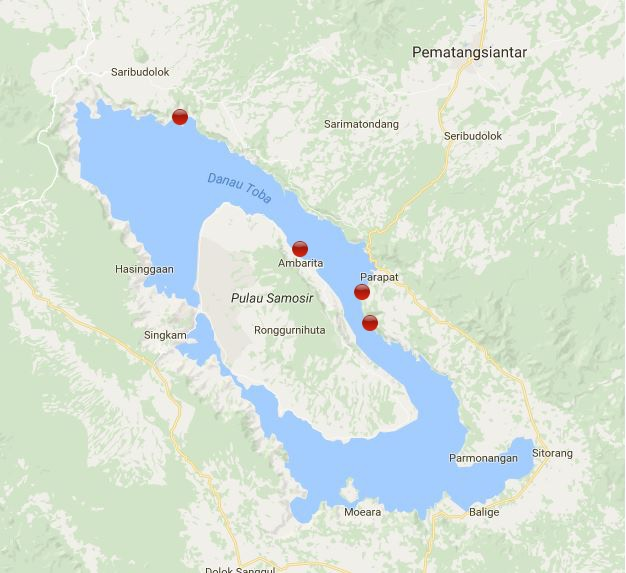
\includegraphics[scale=0.2]{map_data_acquisition.jpg}
\caption{Locations of Data Acquisition \cite{Rahmat16}}
\label{fig1}
\end{figure}

\subsection{General Architecture}

The general architecture of the application is shown by Fig. 2. The development of the application is done in combination of Python and MATLAB environment.

\begin{figure}[!th]
\centering
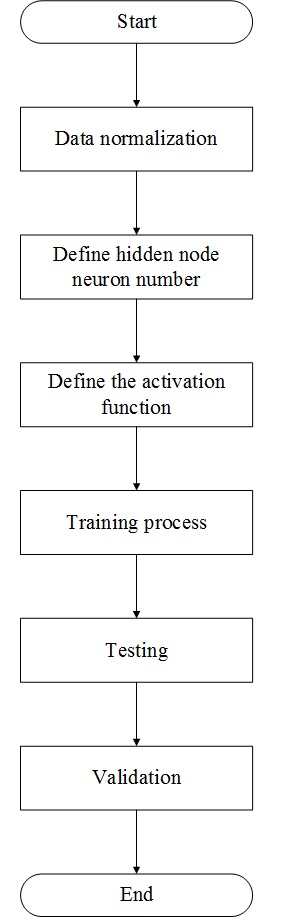
\includegraphics[scale=0.2]{general_architecture.jpg}
\caption{General Architecture of the Application}
\label{fig2}
\end{figure}

The general architecture of the application consists of six steps, which are explained as follows:

\begin{enumerate}

\item Data normalization: The water quality data is recorded by Rahmat {\it et al.} \cite{Rahmat16} by the format shown by Fig 3. The recorded values are separated by semicolon sign, thus needs rearrangement and normalization. According to Patro {\it et al.} \cite{Patro15} , normalization is a pre-processing stage of the problem sets, by which the data will be scaled by the certain range, in order to enable the algorithm to work.

\begin{figure}[!th]
\centering
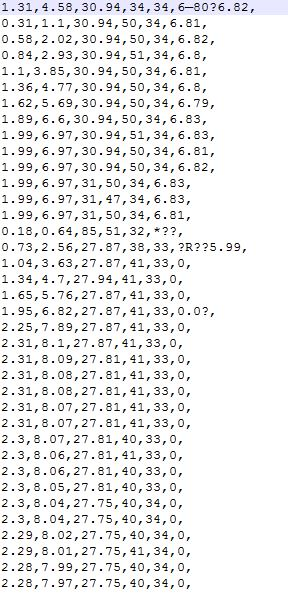
\includegraphics[scale=0.2]{fig-3.jpg}
\caption{Initial Data Structure\cite{Rahmat16}}
\label{fig3}
\end{figure}

\item Define the number of hidden neuron: This process will be performed after data normalization process is done. According to Heaton \cite{Heaton08} , the number of hidden neuron has to be defined by using following rules:

\begin{itemize}
\item the number of hidden neuron ranges from the number of input neuron and the number of output neuron,
\item the number of hidden neuron can be defined as two thirds of the total input and output neuron, and
\item the number of hidden neuron is not higher than twice the number of input neuron
\end{itemize}

Various amount of hidden neuron will be implemented in this research for comparation of the prediction result. The number of hidden neuron varies from 1 to 20.

\item Define the activation function: Dorst \cite{Dorst16} defines the activation function is the function implemented in the neuron to determine the state of the neuron in an artificial neural network. In this research, three activation functions will be implemented, respectively sigmoid, sine, and hardlim function, whose result will be compared.

\item Training process: The training process is a process performed in artificial neural network implementation. The training process is performed by using extreme learning machine in the following steps:

\begin{itemize}
\item Initialize the hidden layer matrix $H$, consisting of input weights and neuron biases;
\item Calculate the hidden layer output from matrix $H$;
\item Calculate output weight matrix $\beta$, which is done according to (4).
\end{itemize}

\item Testing process: The testing process is performed after the training process is done. The testing process is performed to obtain the result of training process.

\item Validation process: The validation process is performed after the testing process is done. The validation process is performed to verify that the result generated in testing process conforms with the water quality index standard.

\end{enumerate}

The output of the methodology in this research is a graph representing the result of prediction process by the extreme learning machine, followed by the root mean square error and the calculation time of the result.

\section{Experiment and Result}

The process of water quality prediction is done through combination of Python and MATLAB environment. The data normalization process is done through Python environment, while the water quality prediction process is performed through MATLAB environment.

\subsection{Data Normalization}

The data normalization process is done through Python environment. The initial data structure is not suitable to be processed with extreme learning machine, thus requiring normalization process.

Before the data is normalized, the initial dataset have to be filtered by each row, to ensure that the value of the recorded data is a valid numeric data. The result of the filtering process is a new dataset with valid numeric value.

The normalization process is performed by using min-max normalization \cite{Patro15} , thus resulting in a dataset with value ranging from -1 to 1, according to \eqref{Eq. 5}:

\begin{equation}
A' = \frac{A - A_{min}}{A_{max} - A_{min}} * (D - C) + C\label{Eq. 5}
\end{equation}

where $A'$ refers to the normalized data value of $A$, with the result ranging from $[C, D]$. The result of the normalization process will be used by the extreme learning machine regression engine \cite{Zhu13}.

\subsection{Water quality prediction}

The water quality prediction process is done through MATLAB environment. The interface of the system is shown in Fig 4.

\begin{figure}[!th]
\centering
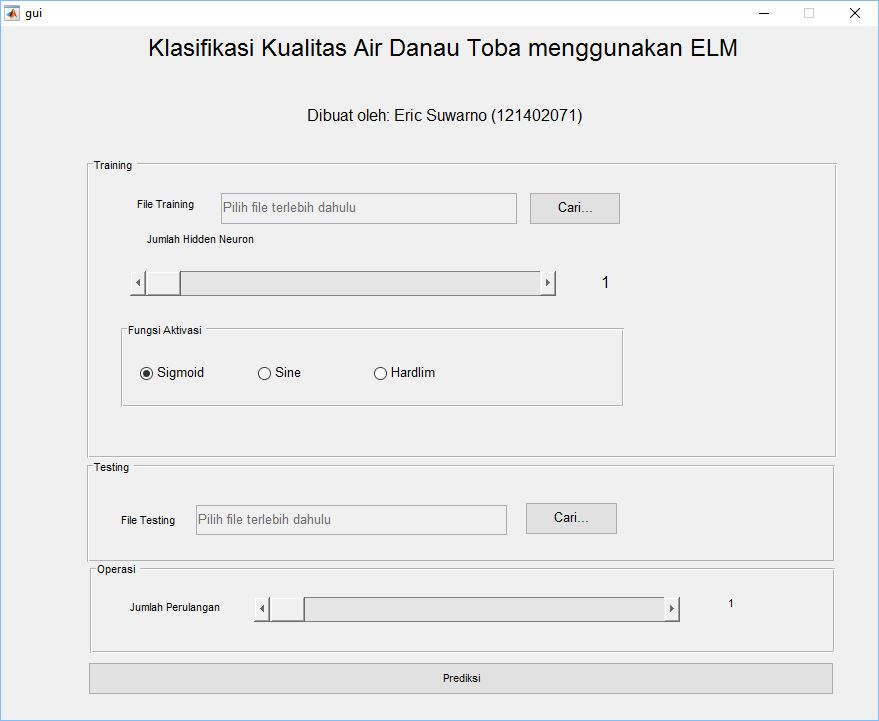
\includegraphics[scale=0.2]{fig-4.jpg}
\caption{The Appearance of the System}
\label{fig4}
\end{figure}

To perform the water quality prediction process, the training data and testing data have to be provided to the system. The default architecture of the artificial neural network, which will be constructed after training data is loaded, is SLFN with sigmoid function as the activation function. The number of hidden neuron is set to 1 by default, with the range of 1 to 20. The result of the water quality prediction process is shown in a graph, showing training error rate, training time, testing error time, and testing time. The appearance of the result view is shown in Fig 5.

% figure 5
%\begin{figure}[!th]
%\centering
%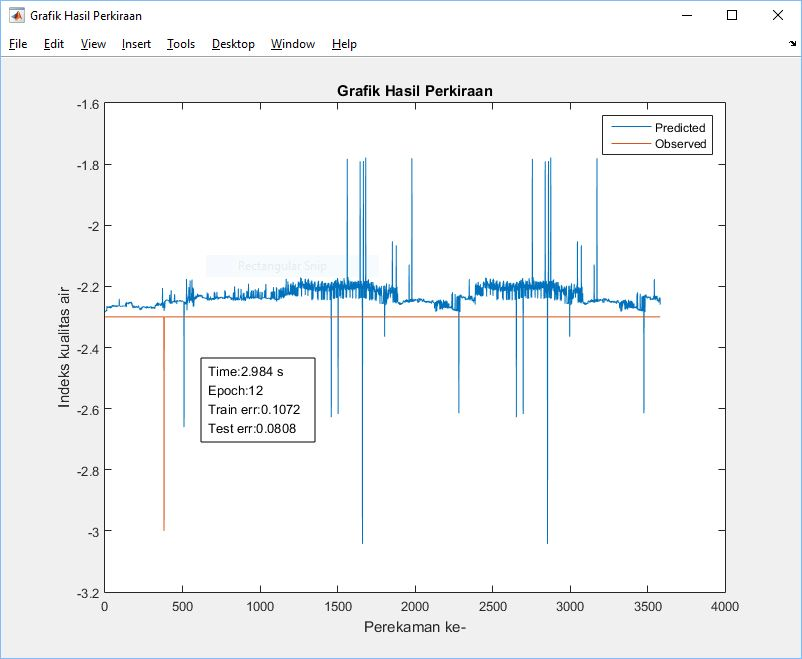
\includegraphics[scale=0.2]{fig-5.jpg}
%\caption{The Appearance of the Prediction Result}
%\label{fig4}
%\end{figure}

    \[Silakan~tulis~hasil~penelitian~di~sini.\]

% needed in second column of first page if using \IEEEpubid
%\IEEEpubidadjcol

%\subsubsection{Subsubsection Heading Here}
%Subsubsection text here.


% An example of a floating figure using the graphicx package.
% Note that \label must occur AFTER (or within) \caption.
% For figures, \caption should occur after the \includegraphics.
% Note that IEEEtran v1.7 and later has special internal code that
% is designed to preserve the operation of \label within \caption
% even when the captionsoff option is in effect. However, because
% of issues like this, it may be the safest practice to put all your
% \label just after \caption rather than within \caption{}.
%
% Reminder: the "draftcls" or "draftclsnofoot", not "draft", class
% option should be used if it is desired that the figures are to be
% displayed while in draft mode.
%
%\begin{figure}[!t]
%\centering
%\includegraphics[width=2.5in]{myfigure}
% where an .eps filename suffix will be assumed under latex, 
% and a .pdf suffix will be assumed for pdflatex; or what has been declared
% via \DeclareGraphicsExtensions.
%\caption{Simulation results for the network.}
%\label{fig_sim}
%\end{figure}

% Note that the IEEE typically puts floats only at the top, even when this
% results in a large percentage of a column being occupied by floats.


% An example of a double column floating figure using two subfigures.
% (The subfig.sty package must be loaded for this to work.)
% The subfigure \label commands are set within each subfloat command,
% and the \label for the overall figure must come after \caption.
% \hfil is used as a separator to get equal spacing.
% Watch out that the combined width of all the subfigures on a 
% line do not exceed the text width or a line break will occur.
%
%\begin{figure*}[!t]
%\centering
%\subfloat[Case I]{\includegraphics[width=2.5in]{box}%
%\label{fig_first_case}}
%\hfil
%\subfloat[Case II]{\includegraphics[width=2.5in]{box}%
%\label{fig_second_case}}
%\caption{Simulation results for the network.}
%\label{fig_sim}
%\end{figure*}
%
% Note that often IEEE papers with subfigures do not employ subfigure
% captions (using the optional argument to \subfloat[]), but instead will
% reference/describe all of them (a), (b), etc., within the main caption.
% Be aware that for subfig.sty to generate the (a), (b), etc., subfigure
% labels, the optional argument to \subfloat must be present. If a
% subcaption is not desired, just leave its contents blank,
% e.g., \subfloat[].


% An example of a floating table. Note that, for IEEE style tables, the
% \caption command should come BEFORE the table and, given that table
% captions serve much like titles, are usually capitalized except for words
% such as a, an, and, as, at, but, by, for, in, nor, of, on, or, the, to
% and up, which are usually not capitalized unless they are the first or
% last word of the caption. Table text will default to \footnotesize as
% the IEEE normally uses this smaller font for tables.
% The \label must come after \caption as always.
%
%\begin{table}[!t]
%% increase table row spacing, adjust to taste
%\renewcommand{\arraystretch}{1.3}
% if using array.sty, it might be a good idea to tweak the value of
% \extrarowheight as needed to properly center the text within the cells
%\caption{An Example of a Table}
%\label{table_example}
%\centering
%% Some packages, such as MDW tools, offer better commands for making tables
%% than the plain LaTeX2e tabular which is used here.
%\begin{tabular}{|c||c|}
%\hline
%One & Two\\
%\hline
%Three & Four\\
%\hline
%\end{tabular}
%\end{table}


% Note that the IEEE does not put floats in the very first column
% - or typically anywhere on the first page for that matter. Also,
% in-text middle ("here") positioning is typically not used, but it
% is allowed and encouraged for Computer Society conferences (but
% not Computer Society journals). Most IEEE journals/conferences use
% top floats exclusively. 
% Note that, LaTeX2e, unlike IEEE journals/conferences, places
% footnotes above bottom floats. This can be corrected via the
% \fnbelowfloat command of the stfloats package.




\section{Conclusion}
The water quality prediction is done by implementing extreme learning machines (ELM), based on the water quality data recorded by Rahmat {\it et al.} \cite{Rahmat16} , by applying different variations of activation functions and number of hidden neurons.






% if have a single appendix:
%\appendix[Proof of the Zonklar Equations]
% or
%\appendix  % for no appendix heading
% do not use \section anymore after \appendix, only \section*
% is possibly needed

% use appendices with more than one appendix
% then use \section to start each appendix
% you must declare a \section before using any
% \subsection or using \label (\appendices by itself
% starts a section numbered zero.)
%


%\appendices
%\section{Proof of the First Zonklar Equation}
%Appendix one text goes here.

% you can choose not to have a title for an appendix
% if you want by leaving the argument blank
%\section{}
%Appendix two text goes here.


% use section* for acknowledgment
%\section*{Acknowledgment}
%
%
%The authors would like to thank...
%

% Can use something like this to put references on a page
% by themselves when using endfloat and the captionsoff option.
\ifCLASSOPTIONcaptionsoff
  \newpage
\fi



% trigger a \newpage just before the given reference
% number - used to balance the columns on the last page
% adjust value as needed - may need to be readjusted if
% the document is modified later
%\IEEEtriggeratref{8}
% The "triggered" command can be changed if desired:
%\IEEEtriggercmd{\enlargethispage{-5in}}

% references section

% can use a bibliography generated by BibTeX as a .bbl file
% BibTeX documentation can be easily obtained at:
% http://mirror.ctan.org/biblio/bibtex/contrib/doc/
% The IEEEtran BibTeX style support page is at:
% http://www.michaelshell.org/tex/ieeetran/bibtex/
%\bibliographystyle{IEEEtran}
% argument is your BibTeX string definitions and bibliography database(s)
%\bibliography{IEEEabrv,../bib/paper}
%
% <OR> manually copy in the resultant .bbl file
% set second argument of \begin to the number of references
% (used to reserve space for the reference number labels box)
\begin{thebibliography}{1}

%\bibitem{IEEEhowto:kopka}
%H.~Kopka and P.~W. Daly, \emph{A Guide to \LaTeX}, 3rd~ed.\hskip 1em plus
  %0.5em minus 0.4em\relax Harlow, England: Addison-Wesley, 1999.
  
\bibitem{Haro13}
D.~Haro, Y.~Djayus and Z.~Harahap, \textquotedblleft Kondisi Kualitas Air
  Danau Toba di Kecamatan Haranggaol Horison Kabupaten Simalungun Sumatera
  Utara\textquotedblright , {\it AQUACOASTMARINE}, vol. 1, no. 1, 2013.

\bibitem{Lara99}
B.~Lara, K.~Althoefer and D.~Seneviratne, \textquotedblleft Use of artificial neural networks for the monitoring of screw insertions,\textquotedblright {\it Proceedings 1999 IEEE/RSJ International Conference on Intelligent Robots and Systems. Human and Environment Friendly Robots with High Intelligence and Emotional Quotients (Cat. No.99CH36289)}, \hskip 1em plus
  0.5em minus 0.4em\relax Kyongju, 1999, pp. ~579--584 vol.1.
  
\bibitem{Popovic98}
D.~Popovi\' c, D.~Kukolj, and F.~Kuli\' c, \textquotedblleft Monitoring and assessment of voltage stability margins using artificial neural networks with a reduced input set,\textquotedblright \ {\it IEE Proceedings - Generation, Transmission and Distribution}, vol. 145, no. 4, p. ~355--362, 1998.

\bibitem{Ata15}
R.~Ata, \textquotedblleft Artificial neural networks applications in wind 
  energy systems: A review,\textquotedblright \hskip 1em plus
  0.5em minus 0.4em\relax \ {\it Renewable and Sustainable Energy Reviews}, vol. 49,
  pp. ~534--562, Sep. 2015.
  
\bibitem{Shibata09}
K.~Shibata and Y.~Ikeda, \textquotedblleft Effect of number of hidden neurons 
  on learning in large-scale layered neural networks,\textquotedblright \hskip 1em plus
  0.5em minus 0.4em\relax in {\it ICCAS-SICE}, Fukuoka: IEEE, 2009, pp. ~5008--5013.

\bibitem{Deng15}
C.~Deng, G.~Huang, J.~Xu, and J.~Tang, \textquotedblleft Extreme learning
  machines: New trends and applications,\textquotedblright \hskip 1em plus
  0.5em minus 0.4em\relax {\it Science China Information Sciences},
  vol. 58, no. 2, pp. ~020301:1--020301:16, Jan. 2015.

\bibitem{Werbos74}
P.~Werbos. \textquotedblleft Beyond regression: new tools for prediction and 
  analysis in the behavioral sciences,\textquotedblright \hskip 1em plus
  0.5em minus 0.4em\relax Harvard University, Cambridge, Massachusets, 1974.

\bibitem{Rumelhart86}
D.~E. Rumelhart, G.~E. Hinton, and R.~J. Williams, \textquotedblleft Learning
  representations by back-propagating errors,\textquotedblright \hskip 1em plus
  0.5em minus 0.4em\relax {\it Nature}, vol. 323, no. 6088, pp. ~533--536, Oct. 1986.

\bibitem{Chandra14}
B.~Chandra and R.~K. Sharma, \textquotedblleft Fast learning for
  big data applications using parameterized multilayer perceptron,\textquotedblright \hskip 1em plus
  0.5em minus 0.4em\relax \ {\it 2014 IEEE International Conference on 
  Big Data (Big Data)}, pp. ~17--22, 2014.

\bibitem{Chandra16}
B.~Chandra, and R.~K. Sharma. \textquotedblleft Fast learning in
  Deep Neural Networks.\textquotedblright \hskip 1em plus
  0.5em minus 0.4mm\relax \ {\it Neurocomputing}, vol. 171, pp. ~1205--1215, 2016.

\bibitem{Hinton06}
G.~E. Hinton, S.~Osindero, and Y.-W.~Teh, \textquotedblleft A fast
  learning algorithm for deep belief nets,\textquotedblright \hskip 1em plus
  0.5em minus 0.4mm\relax \ {\it Neural Computation}, vol. 18, no. 7, pp. ~1527--1554, Jul. 2006.

\bibitem{Huang06}
G.-B.~Huang, Q.-Y.~Zhu, and C.-K.~Siew, \textquotedblleft Extreme
  learning machine: Theory and applications,\textquotedblright \hskip 1em plus
  0.5em minus 0.4mm\relax \ {\it Neurocomputing}, vol. 70, no. 1-3, pp. ~489--501, Dec. 2006.

\bibitem{Fu15}
F.~Huixuan, W.~Yuchao and Z.~Hongmei, \textquotedblleft Ship rolling 
  motion prediction based on extreme learning machine,\textquotedblright \ {\it 
  2015 34th Chinese Control Conference (CCC)}, Hangzhou, 2015, pp. ~3468--3472.

\bibitem{Pangaribuan14}
J.~J. Pangaribuan and Suharjito, \textquotedblleft Diagnosis of diabetes mellitus
  using extreme learning machine,\textquotedblright \hskip 1em plus
  0.5em minus 0.4mm\relax \ {\it 2014 International Conference on Information Technology Systems and Innovation (ICITSI)}, Bandung, 2014, pp. 33--38.

\bibitem{Zhai08}
C.-M.~Zhai and J.-X.~Du, \textquotedblleft Applying extreme learning machine to plant species identification,\textquotedblright \ {\it 2008 International Conference on Information and Automation}, Changsha, 2008, pp. ~879--884.

\bibitem{Rahmat16} R. F. Rahmat, Athmanathan, M. F. Syahputra dan M. S. Lydia, \textquotedblleft Real Time Monitoring System for Water Pollution in Lake Toba,\textquotedblright \ in {\it Proceedings of ICIC 2016}, Lombok, 2016.

\bibitem{Hammerstrom93}
D. Hammerstrom, \textquotedblleft Neural networks at work,\textquotedblright \hskip 1em plus
  0.5em minus 0.4mm\relax in {\it IEEE Spectrum}, vol. 30, no. 6, pp. ~26--32, June 1993.

\bibitem{Uhrig95}
R.~E. Uhrig, \textquotedblleft Introduction to artificial neural networks,\textquotedblright \hskip 1em plus
  0.5em minus 0.4mm\relax \ {\it Industrial Electronics, Control, and Instrumentation, 1995.},
  {\it Proceedings of the 1995 IEEE IECON 21st International Conference on}, Orlando, FL, 
  1995, pp. ~33--37 vol.1.

\bibitem{Reingnold16}
E.~Reingnold and J.~Nightingale,
    \textquotedblleft Training~an~artificial~neural~network,\textquotedblright 
    \ in {\it Artificial~Neural~Networks~Technology},
  University of Toronto. [Online]. Available: 
  http://www.psych.utoronto.ca/users/reingold/courses/ai/cache/neural3.html.
  Accessed: Nov. 18, 2016.

\bibitem{Heeswijk15} M.~van Heeswijk, \textquotedblleft Advances in 
  extreme learning machines,\textquotedblright \hskip 1em plus
  0.5em minus 0.4mm\relax Aalto University, 2015.

\bibitem{Gao14}
M.~Gao, W.~Xu, H.~Fu, M.~Wang and X.~Liang, \textquotedblleft A Novel Forecasting Method for Large-Scale Sales Prediction Using Extreme Learning Machine,\textquotedblright \hskip 1em plus 0.5em minus 0.4mm\relax {\it 2014 Seventh International Joint Conference on Computational Sciences and Optimization}, Beijing, 2014, pp. ~602--606.

\bibitem{Patro15}
Patro, G.~S. Krishna, and K.~Kumar, \textquotedblleft Title: Normalization: A Preprocessing stage,\textquotedblright \hskip 1em plus 0.5em minus 0.4mm\relax 2015. [Online]. Available: http://arxiv.org/abs/1503.06462. Accessed: Jan. 5, 2017.

\bibitem{Heaton08}
J.~Heaton, {\it Introduction to neural networks for Java, 2nd ed}. New York, NY, United States: Heaton Research, United States, 2008.

\bibitem{Dorst16} L.~Dorst, \textquotedblleft Neural activation functions,\textquotedblright \ in {\it Applications of basic mathematics in Computer Science}. [Online]. Available: https://staff.science.uva.nl/l.dorst/math/sigma.pdf. Accessed: Nov. 22, 2016.

\bibitem{Zhu13} Q.-Y.~Zhu and G.-B.~Huang, \textquotedblleft Extreme learning machines,\textquotedblright \ 2013. [Online]. Available: http://www.ntu.edu.sg/home/egbhuang/elm\textunderscore random\textunderscore hidden\textunderscore nodes.html. Accessed: Jan. 5, 2017.

\end{thebibliography}

% biography section
% 
% If you have an EPS/PDF photo (graphicx package needed) extra braces are
% needed around the contents of the optional argument to biography to prevent
% the LaTeX parser from getting confused when it sees the complicated
% \includegraphics command within an optional argument. (You could create
% your own custom macro containing the \includegraphics command to make things
% simpler here.)
%\begin{IEEEbiography}[{\includegraphics[width=1in,height=1.25in,clip,keepaspectratio]{mshell}}]{Michael Shell}
% or if you just want to reserve a space for a photo:

%\begin{IEEEbiography}{Michael Shell}
%Biography text here.
%\end{IEEEbiography}

% if you will not have a photo at all:
%\begin{IEEEbiographynophoto}{John Doe}
%Biography text here.
%\end{IEEEbiographynophoto}

% insert where needed to balance the two columns on the last page with
% biographies
%\newpage

%\begin{IEEEbiographynophoto}{Jane Doe}
%Biography text here.
%\end{IEEEbiographynophoto}

% You can push biographies down or up by placing
% a \vfill before or after them. The appropriate
% use of \vfill depends on what kind of text is
% on the last page and whether or not the columns
% are being equalized.

%\vfill

% Can be used to pull up biographies so that the bottom of the last one
% is flush with the other column.
%\enlargethispage{-5in}



% that's all folks
\end{document}


